\section{The way point system}
\label{sec:wayPointSystem}

\subsection{Concept}

To enable the drivers to see things in the world, we developed a system of 
objects that we call the way points. When a driver looks at it's vicinity, all
things in this area are collected and passed to the driver as way points.\\

\noindent The area that describes what the driver can see is implemented as the 
''driver view`` (\ref{sec:driverView}) and is based on the manner 
how humans view their environment. \\

\noindent To have an efficient filter for the way points we implemented a quad tree 
(\ref{sec:quadTree}).

\subsection{Types of way points}

We thought about the things that a driver would see when driving through a 
street that could have an effect on his behaviour. Such things could be

\begin{itemize}
\item Other vehicles (cars, bicycles, trucks,...)
\item Pedestrians
\item Road signs
\item Junctions
\item Pedestrian crossing
\item ...
\end{itemize}

For this project, we decided to implement only the way points for other
cars, junctions and speed signs, but the design should still be open for 
other way points in a later stage of the project. So we came up with following
class design:

\begin{figure}[htb]
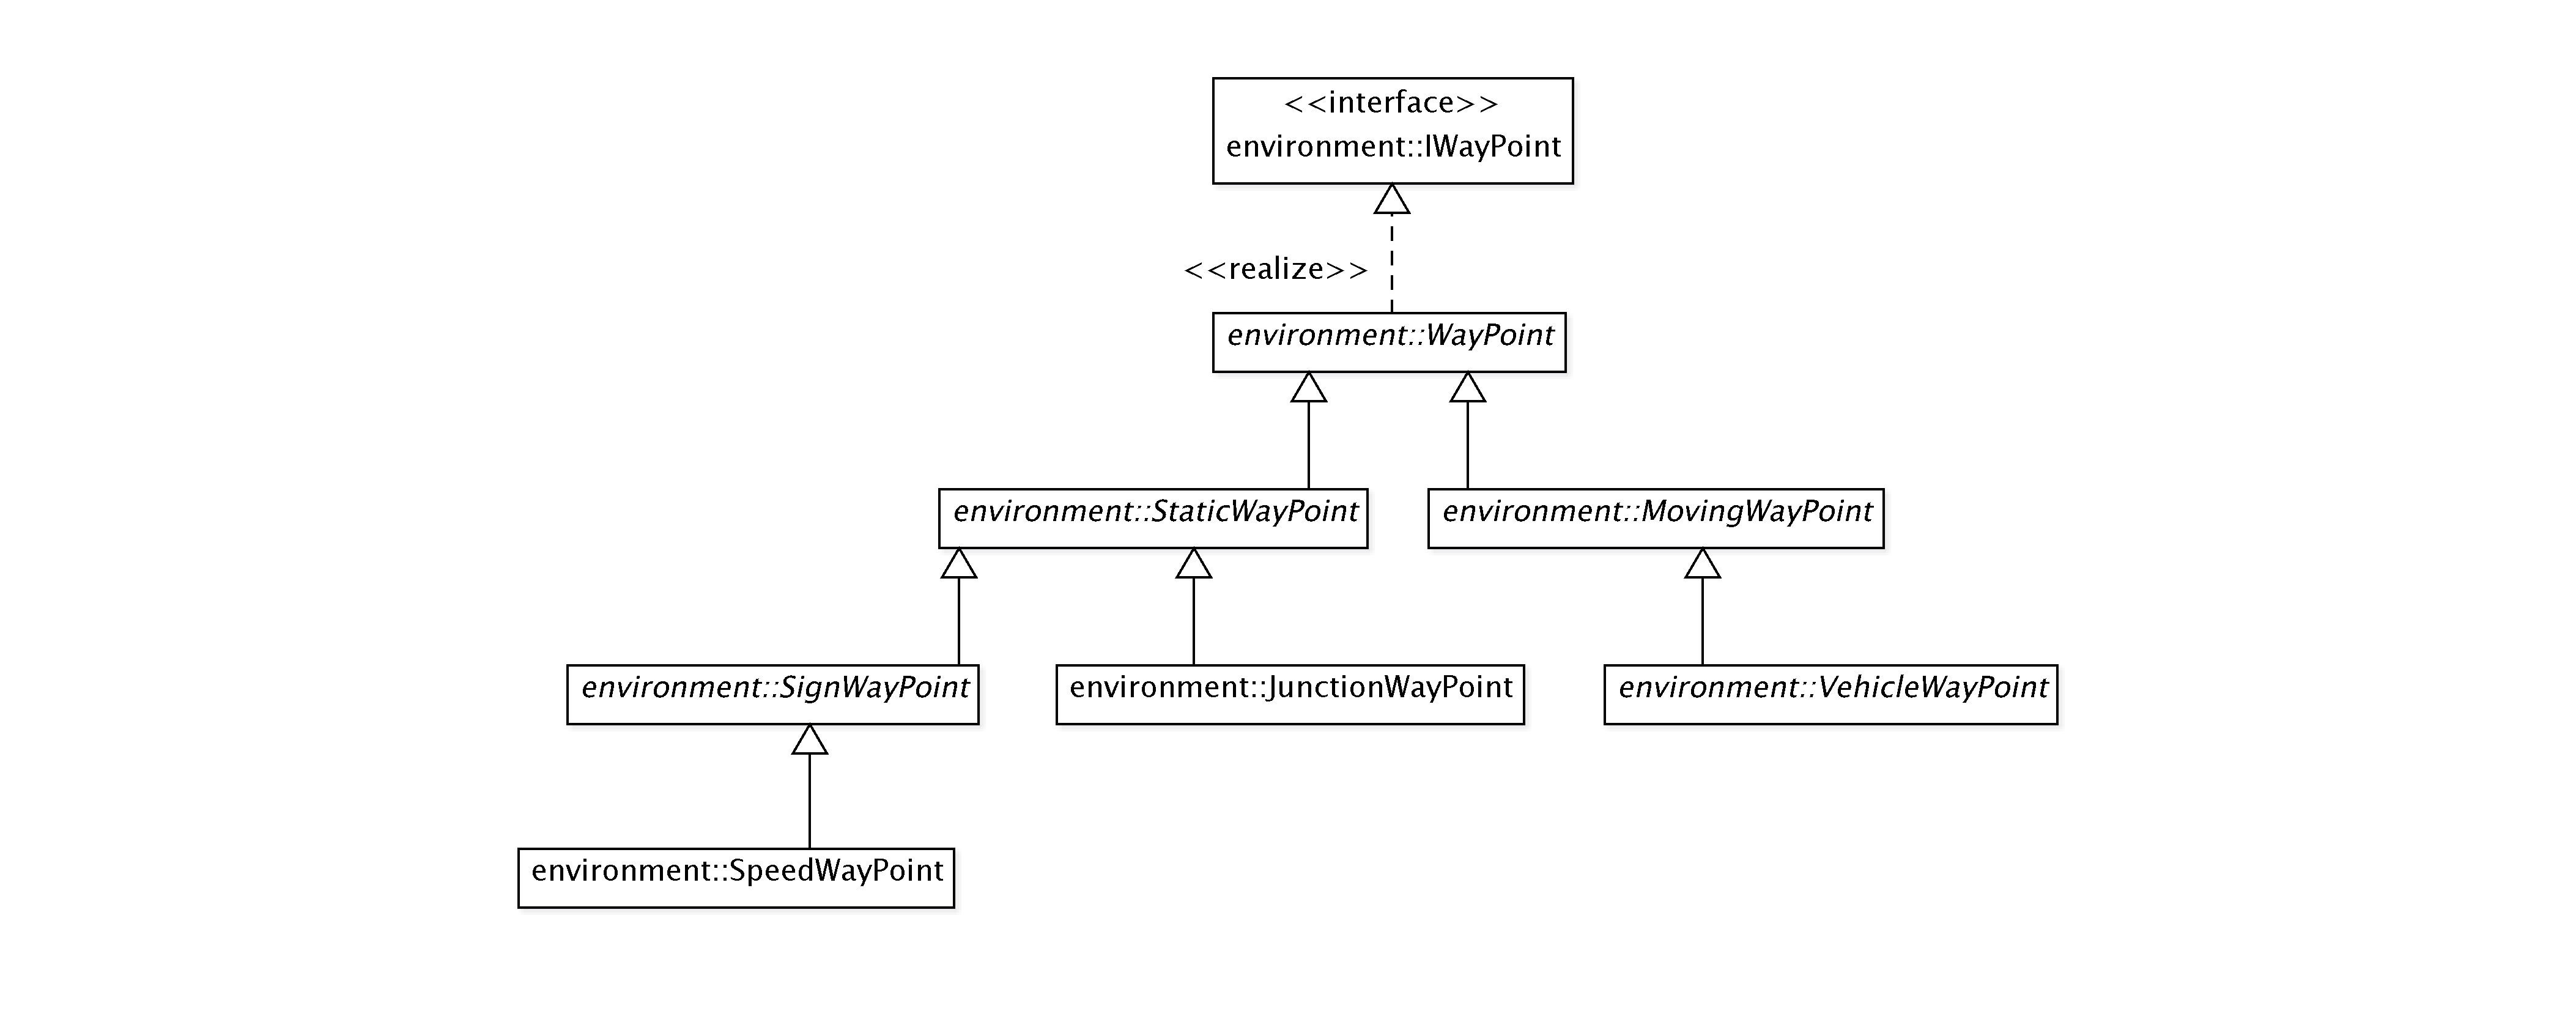
\includegraphics[width=\textwidth]{images/waypoints.png}
\caption{The class design of the way points}
\label{fig:waypoints}
\end{figure}

\noindent The implemented way points are described further below. \\

\label{par:movingWPDistance}
\noindent An important thing to note is that the way points  have a method to 
return the distance to another vehicle. To make it more realistic, some random 
error is added to this distance, since humans can only estimate distances.

\subsubsection{Static way points}

The static way points are those that will never be moved in the world.

\paragraph{Junction way points}
A junction way point describes a junction. It provides the information, in
which directions the driver can go. Junction way points are generated by the
junctions and placed on the lanes (\ref{sec:roadModel}) at 80\% of the lane
length.

\paragraph{Speed way points}
The speed way points are road signs that restrict the speed limit to a certain
value. To keep things simple, there is, unlike in the real world, no sign to 
abrogate the speed limit to the default value. \\

\noindent These way points are given by the XML (\ref{sec:XML}) file that describes the 
world.

\subsubsection{Moving way points}

Some of the way points represent moving objects. Since we only have cars in this
project, only those way points are needed. \\

\paragraph{Car way points}
These way points represent other cars in the simulation. Each car generates its
way point and updates its position as the car moves.

\subsection{Way point finding}

The search for way points that a driver can see is achieved in two steps:

\begin{itemize}
\item Filter with a quad tree
\item Filter with the driver view
\item Check the lanes
\end{itemize}


\subsubsection{The quad tree}
\label{sec:quadTree}

To be able to locate the way points in a certain area quickly, they are 
organized in a quad tree. The quad tree basically divides the world into 
rectangles as shown in figure \ref{fig:quadTree} to a certain depth, which are 
nodes in the tree. The depth defines the resolution of the tree, and depending
on the depth the nodes cover each an area in the world. The nodes 
are created only if there are way points their area. They can contain
more than one way point, since there can be more than one way point in an 
area.\\

\begin{figure}[H]
\begin{center}
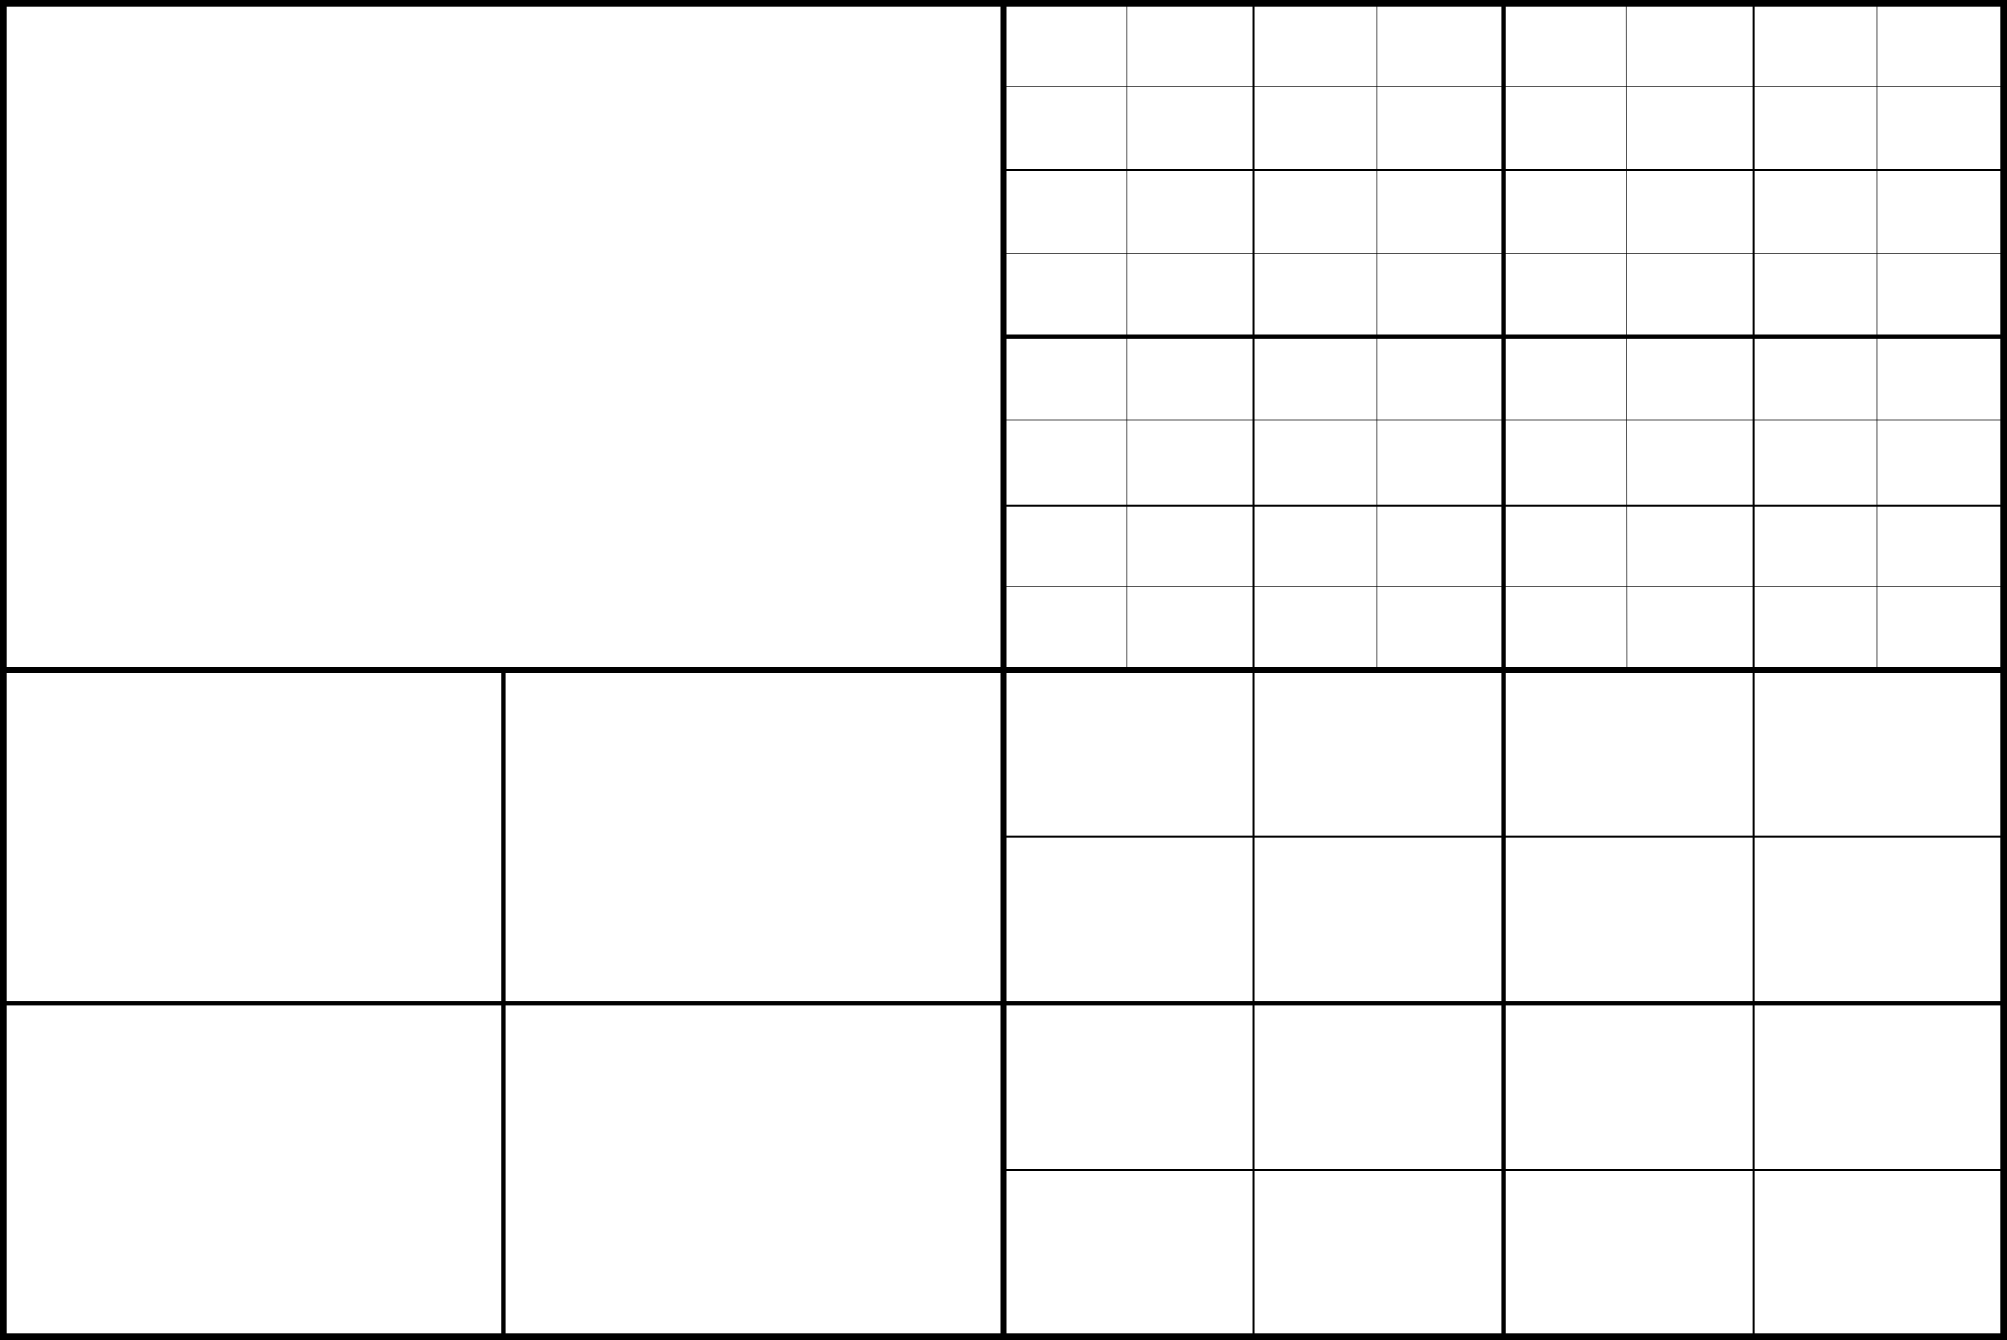
\includegraphics[scale=0.5]{images/quadtree.png}
\end{center}
\caption{A quad tree with the level 4 in the top right corner}
\label{fig:quadTree}
\end{figure}

\noindent With this implementation, all the nodes in the vicinity of the vehicle can be
found with O(d) where d is the depth of the three. Since the quad tree is based
on rectangles, the results have to be filtered further to determine if the located
way points really lie in the driver view, which is explained in the next 
chapter.\\

\noindent Figure \ref{fig:quadTreeClasses} shows the composition of the quad tree classes.

// TODO: mention the moving of way points in the tree

\begin{figure}[H]
\begin{center}
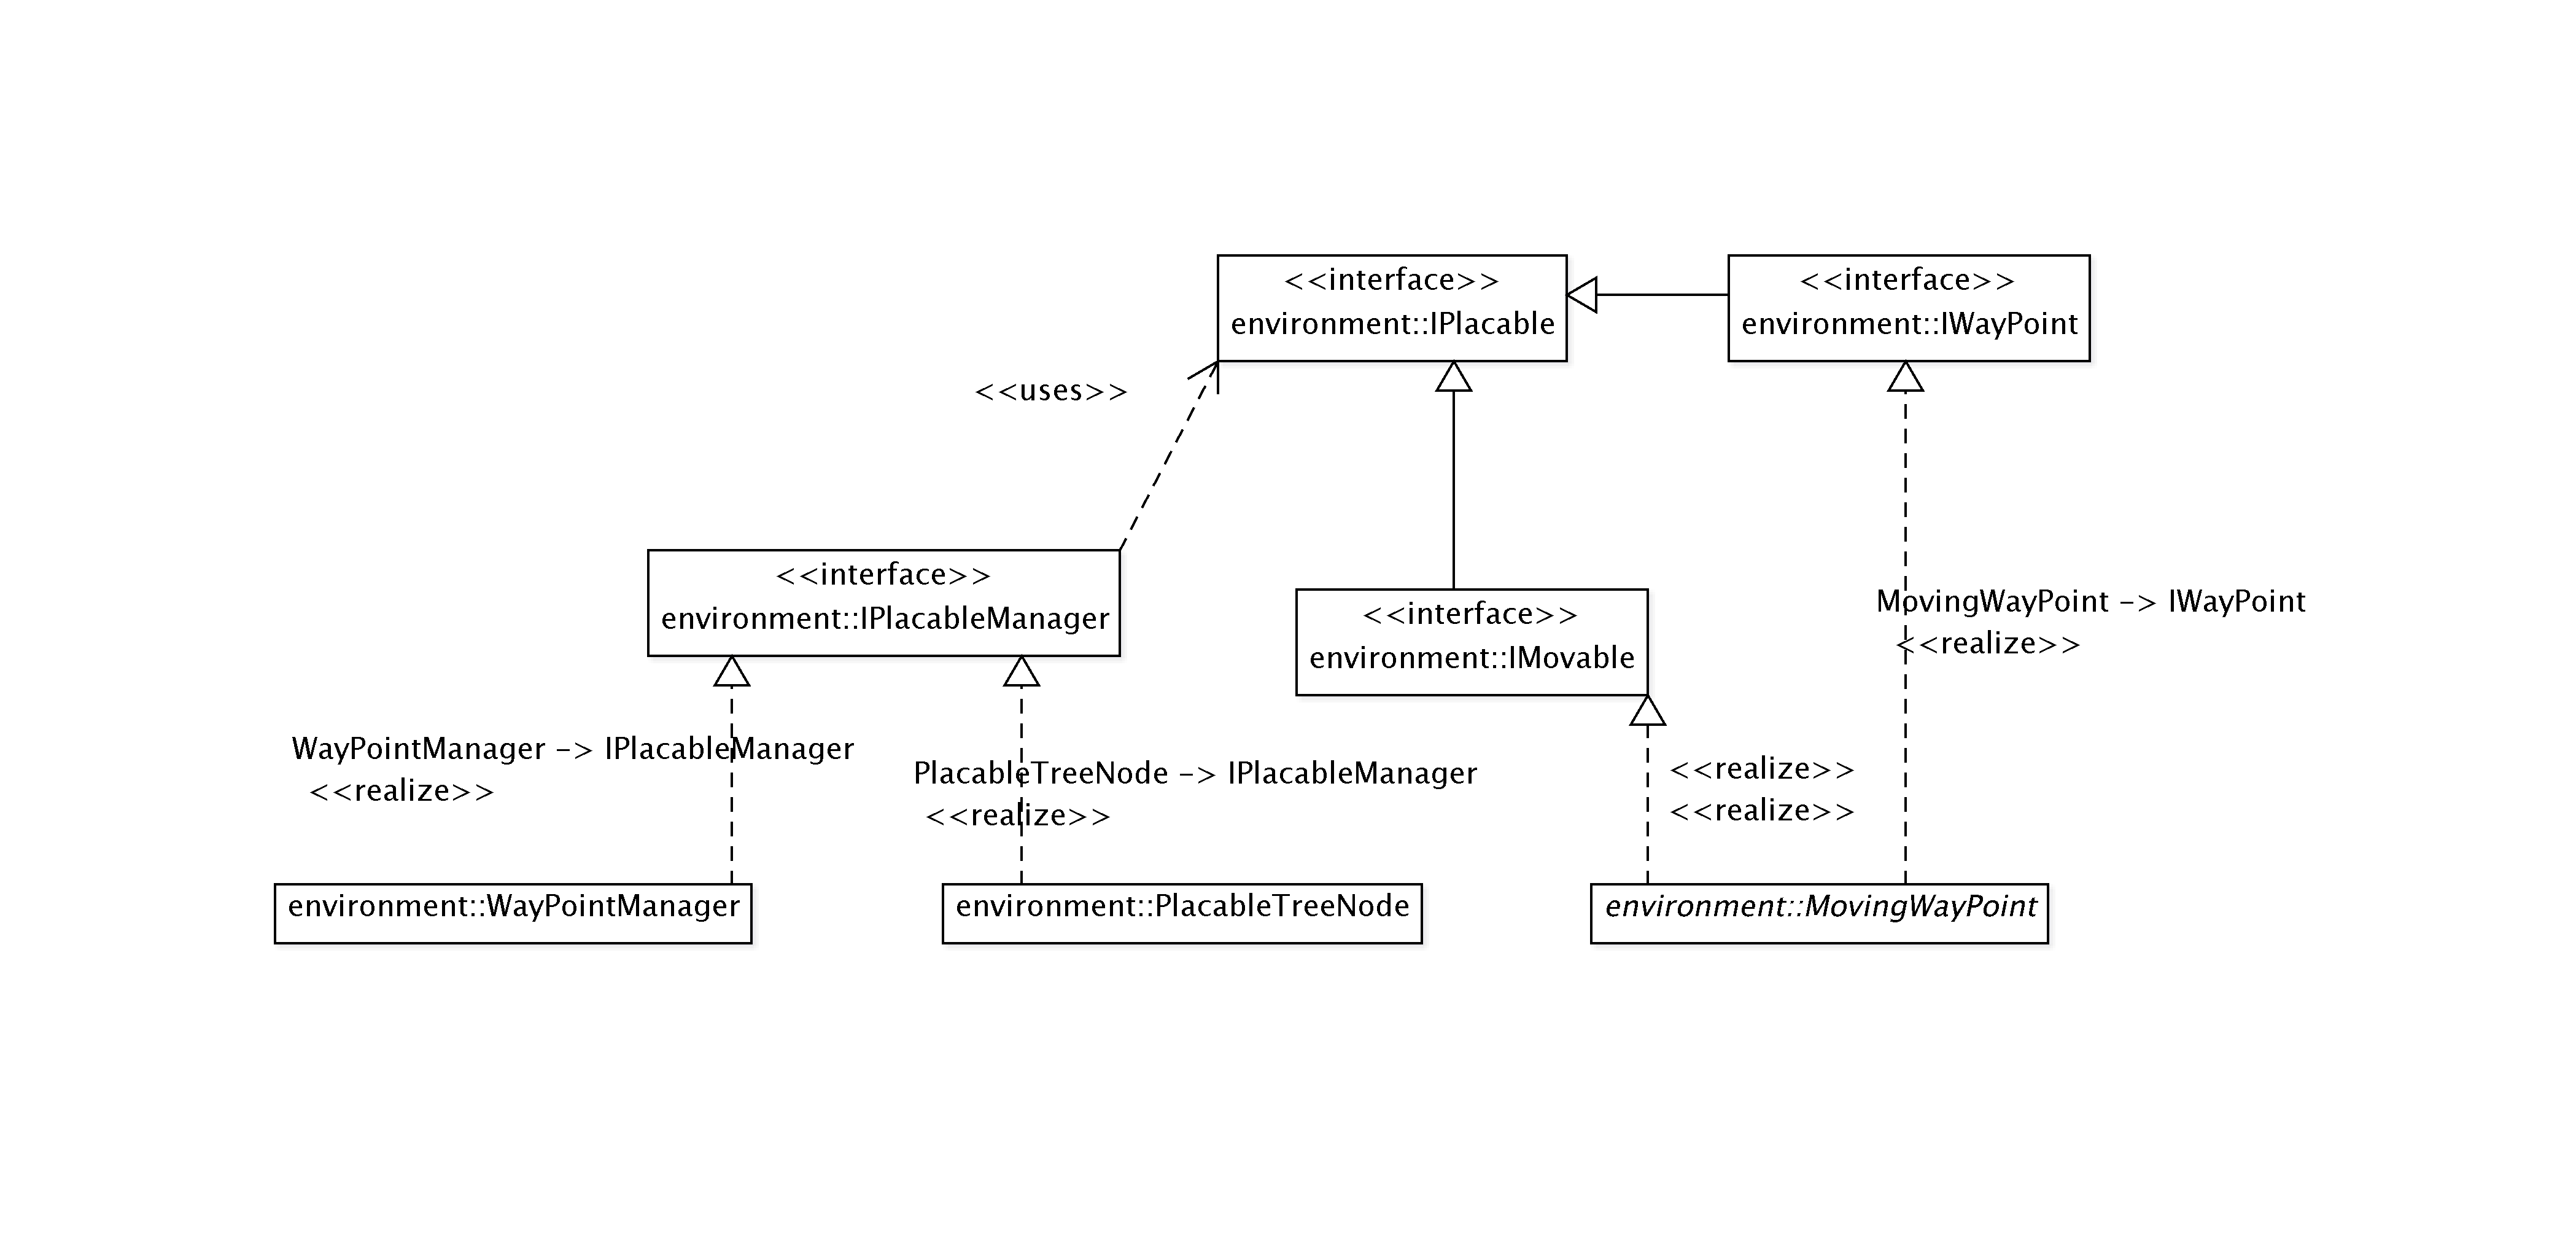
\includegraphics[width=\textwidth]{images/waypointsmanager.png}
\end{center}
\caption{The quad tree classes}
\label{fig:quadTreeClasses}
\end{figure}

\subsubsection{The driver view}
\label{sec:driverView}

\paragraph{Description}

The driver view describes the area wherein the driver can see other objects in
the world. It is described by following parameters:

\begin{itemize}
\item \textbf{Direction} The direction the driver looks
\item \textbf{Position} The position of the driver view 
\item \textbf{Angle} The angle of the visual field
\item \textbf{Distance} The distance that the driver can see
\end{itemize}

\noindent Drugs can be applied to these parameters. They can have a certain effect
on each of the parameters. \\

\noindent With this system of parameters we tried to make the driver view as realistic
as possible. Figure \ref{fig:driverView} depicts the driver view.

\begin{figure}[H]
\begin{center}
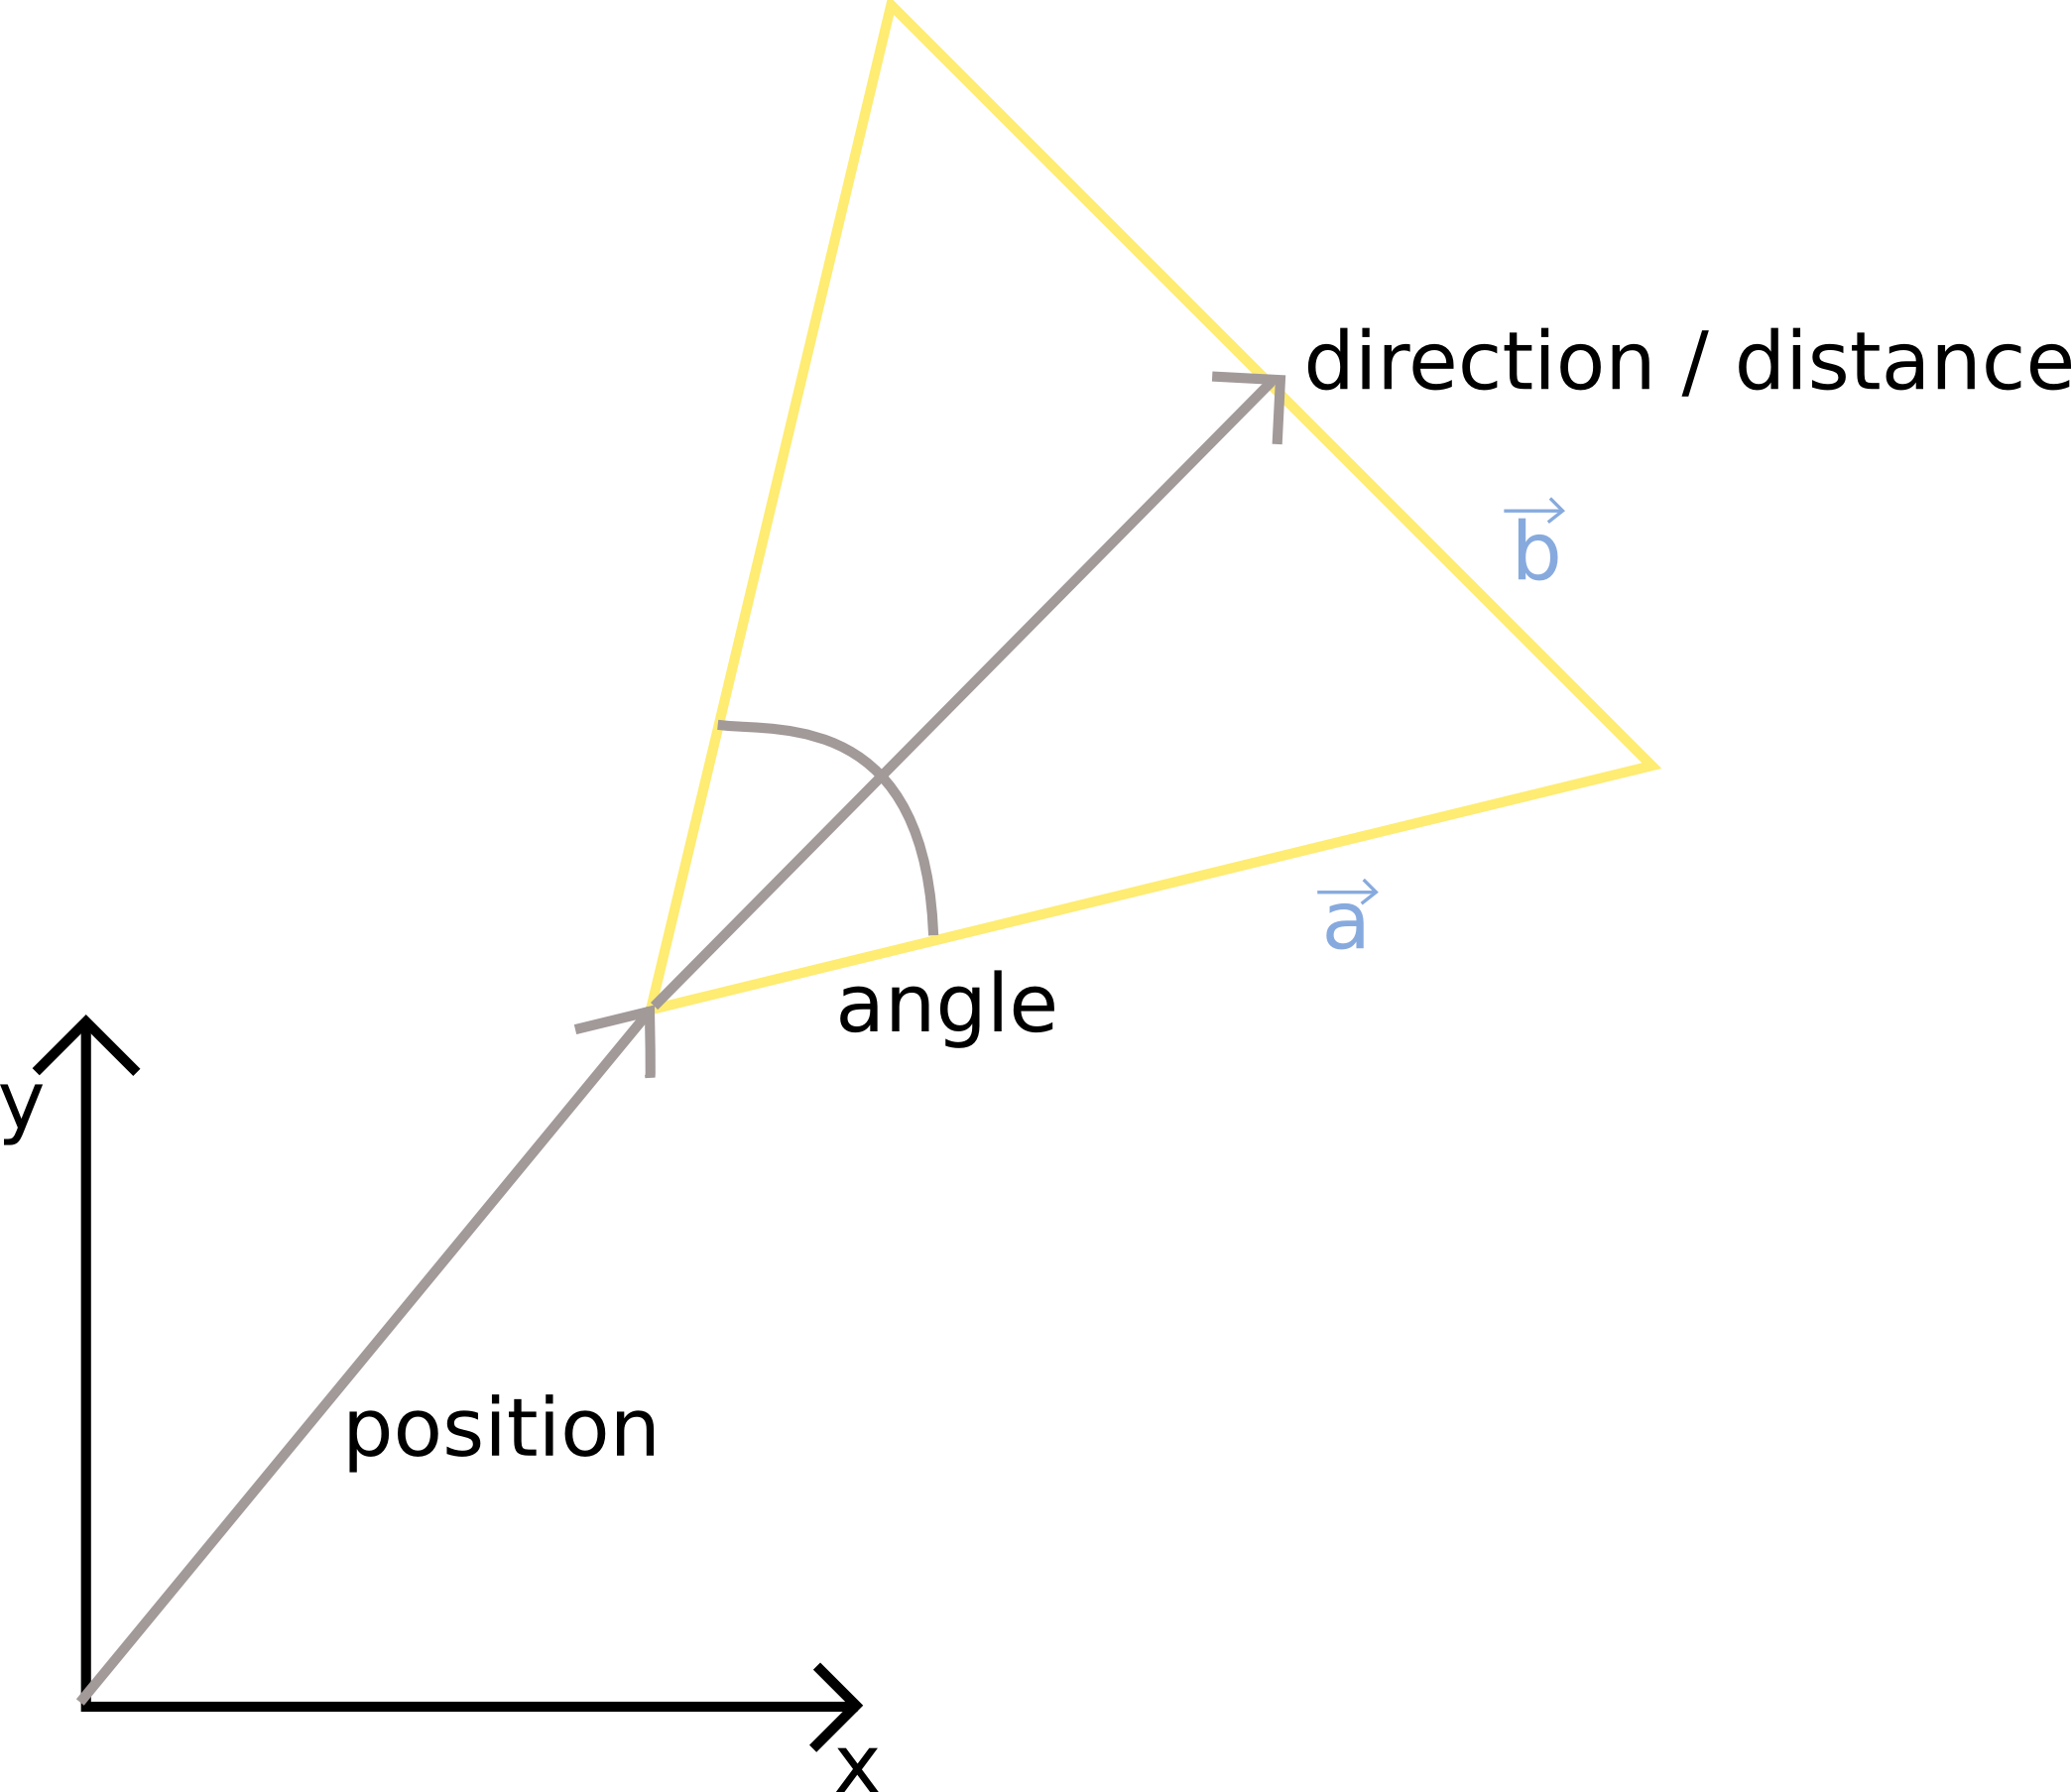
\includegraphics[scale=0.4]{images/driverview.png}
\end{center}
\caption{The driver view}
\label{fig:driverView}
\end{figure}

\paragraph{The filtering}

After the quad tree (\ref{sec:quadTree}) has completed it's search, the located way
points are filtered further to take account of the angled driver view instead
of using just a rectangle. \\

\noindent The algorithm to determine, whether a way point lies in the driver 
view, is based on the following equation: \\

$
\lambda * \vec{a} + \mu * \vec{b}
$ \\

\noindent where $\vec{a}$ is the view boundary to the right of the direction 
vector and $\vec{b}$ is the boundary on top of the view (see figure 
\ref{fig:driverView})). $\lambda$ and $\mu$ are then calculated using the 
vector $\vec{v}$, which is the position of the way point to check, with following
equations: (all vectors are relative to the position of the driver view) \\

$ \lambda = \frac{-(b_x*v_y - b_y * v_x)}{a_x * b_y - a_y * b_x}$\\

$\mu = \frac{a_x * v_y - a_y * v_x}{a_x * b_y - a_y * b_x} $ \\

\noindent If following constraints are fulfilled, the way point lies in the driver
view triangle: \\

$ \lambda, \mu \in ]0, 1]$ \\

$ \frac{\lambda * \left| \vec{b} \right| }{\mu * \left| \vec{a} \right|} \leq 
\frac{\left| \vec{b} \right|}{\left| \vec{a} \right|}$

\paragraph{Further thoughts}
...Some further stuff like the driver view should be adapted when the driver
and how this could be implemented...


\subsubsection{Lane check}

At the last step of way point finding, the way points are checked with the
lane queue of the vehicle (\ref{sec:laneChanges}). If the way point is not
on any of the lanes in the vehicle's queue, it is dropped, since it doesn't
concern the driver. An example of such a way point is a vehicle on the lane
that goes in the opposite direction of the road.
